
%-------------------------------------------------------------------------------
\section{Background}
%-------------------------------------------------------------------------------

Our approach to program analysis draws on work in three fields: Dataflow Analyis on Programs, Nonsmooth Optimization, and Automatic Differentiation. Dataflow Analysis models the flow of data through a program by tracking variable interactions and has applications in both compiler optimization and detection of security vulnerabilities, but suffers from high false positive rates that limit its utility. Nonsmooth Gradient Approximation involves a collection of methods that have been developed in the field of Nonsmooth Optimization for approximating gradients in cases where the gradient cannot be evaluated analytically. These methods make it possible to approximate gradients on discrete and nonsmooth functions in a principaled way based on the local behavior of the function. Finally, we draw on the field of Automatic Differentiation, which involves methods for computing gradients over programs compused of semi smooth numerical operations, but not general programs with discrete and nonsmooth operations.


\subsection{Definitions}


\subsection{Dataflow Analysis}

Dataflow analysis is a form of program analysis that models which variables can effect each other through a program, thereby tracking the flow of data. Typically, dataflow analysis is performed by using a set of rules for which inputs can effect which outputs for each operation. Then program variables, typically inputs, are marked with labels that are propogated through the program via the predefined rules so that internal program variables are labeled with variables that can potentially affect them. 

Static dataflow analysis has been used as a tool for program analysis since it was first introduced in early 1970s ~\cite{kildall1973unified}. However, while it is useful for tasks like compile time optimization, its utility for detecting potential vulnerabilities is limited because it cannot distinguish impossible execution paths, resulting in high false positive rates. Dynamic dataflow analysis, or taint analysis, limits itself to possible executionsby operating on concrete inputs ~\cite{newsome2005dynamic}, but still suffers from high false positive rates caused by overapproximations such as the shift overapproximation shown in figure \ref{fig:taint_v_gradient}. These overapproximations in aggregate result in many inputs incorrectly being flagged as affecting taint sinks, which still limits the utility of taint analysis.

\begin{figure*}[t]
  \centering
  \begin{subfigure}[b]{0.32\textwidth}
    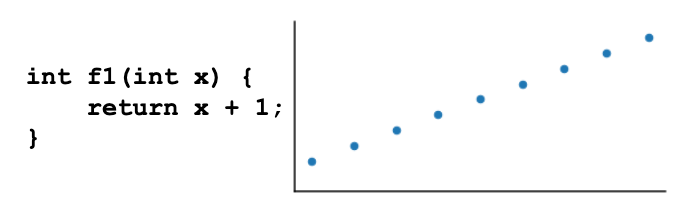
\includegraphics[width=\textwidth]{figs/f1}
  \end{subfigure}
  \begin{subfigure}[b]{0.32\linewidth}
    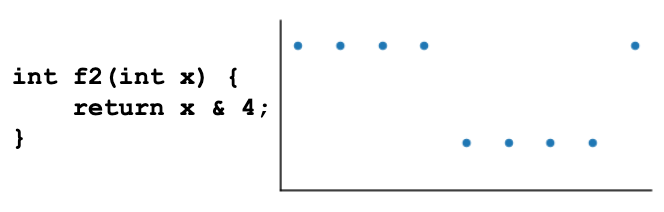
\includegraphics[width=\linewidth]{figs/f2}
  \end{subfigure}
  \begin{subfigure}[b]{0.32\linewidth}
    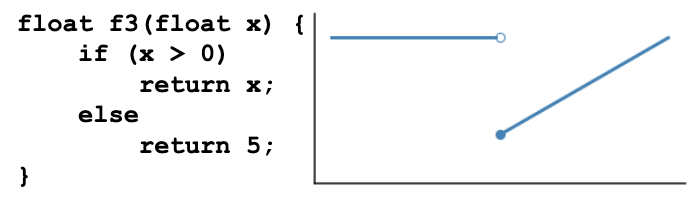
\includegraphics[width=\linewidth]{figs/f3}
  \end{subfigure}
  \vspace{-10pt}
   \caption{ Types of discrete and nonsmooth operations that occur in programs. \tc{f1} is a linear function that is still not differentiable because it operates on integers, while \tc{f2} performs bitwise \tc{and}, which is both discrete and nonsmooth. \tc{f3} illustrates a discontinuity due to branching and merging.}
  \label{fig:ex_funcs}
  \vspace{-10pt}
\end{figure*}

\subsection{Nonsmooth Gradient Approximation}

Programs are inherently difficult to differentiate because their behavior is generally discrete and nonsmooth, meaning that they cannot be differentiated directly. This behavior comes primarily from branches and memory operations, but also from many discrete operations such bitwise operators and integer arithmetic. Figure ~\ref{fig:ex_funcs} gives three examples of different types of operations that are difficult to differentiate. \tc{f1} is a simple linear function, but still is not analytically differentiablebecause it operates on integers and is discrete. \tc{f2} is also discrete, but introduces additional nonsmoothness with a \tc{and} operation. \tc{f3} shows how even on floating point operations branching can result in nonsmooth behavior.

Fortunately, extensive work has been done in the field of optimization on methods for approximating gradients over discrete and nonsmooth functions. The type of approximation that used depends on whether the function is convex, meaning that any point on the function can be connected to any other point by a straight line without going 'under' the function. Operations like addition and multiplication, or multiplying a variable by itself, are convex, but bitwise operations and discontinuities from branching generally are not. When the functions being analyzed are convex, a type of gradient approximation called subgradients may be used that behave similarly to gradients on smooth functions with regard to composition and global convergence properties. When functions are nonconvex, an extension of subgradients called generalized gradients may be used that allow optimization to still be performed, although they relax the composition and convergence properties of subgradients ~\cite{clarke1990optimization, rockafellar2009variational}.

\begin{figure}
  \centering
  \begin{subfigure}[b]{0.48\columnwidth}
    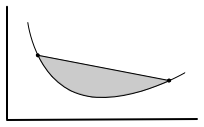
\includegraphics[width=\linewidth]{figs/convex_example}
    \caption{\label{fig:convex_ex} Convex function. Any line between two points on the function will pass 'over' the function.}
  \end{subfigure}
  \hspace{0.15cm}
  \begin{subfigure}[b]{0.48\columnwidth}
    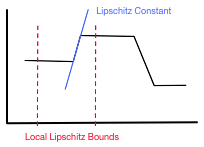
\includegraphics[width=\linewidth]{figs/lipschitz_ex}
  \caption{\label{fig:lipschitz_ex} Function with local Lipschitz Constant.}
  \end{subfigure}
  \vspace{-10pt}
  \caption{\label{fig:convex_lip_ex} Subgradient and Generalized Derivative examples.}
  \vspace{-15pt}
\end{figure}

\noindent \textbf{Convex Gradient Approximation.} Subgradients have been used in these cases to successfully optimize a wide variety of nonsmooth problems when the functions involved were convex ~\cite{beck2017first}. Subgradients are defined to be any vector under a convex function that intersects the function at the point the subgradient is evaluated, or formally, a vector $v$ is a subgradient of a function $f$ at a point $\bar{x}$ if:

\vspace{-10pt}\begin{align}
  f\left(x\right) \geq f\left(\bar{x}\right) + \langle v, x-\bar{x} \rangle \textrm{ for all } x \in \textrm{dom}\left(f\right)
\end{align}

This definition means that any point on the subgradient vector $v$ ($\langle v, x-\bar{x}$) for which $f$ is defined ($x \in \textrm{dom}\left(f\right)$), the value of the subgradient starting from the point it touches the function $f$ can continue to touch $f$ but can never be greater than $f$. This means that there can actually multiple subgradients for a given point of a discrete convex function, as in the example in figure \ref{fig:subgradient}. It is important to note that subgradients can also be defined in terms of being greater than the function in the case one wants to find the highest values of $f$, but conventionally used with vectors under the surface of a function. 

Subgradients are valid for discrete functions and thus can be computed on integer operations like \tc{f1} in figure \ref{fig:ex_funcs}. The chain rule also applies to them, meaning that subgradients of several sequential operations can be multiplied together to give a valid subgradient for combined operations.

\noindent \textbf{Nonconvex Gradient Approximation.} Nonconvex operations (which have multiple minima and maxima) like \tc{and} in \tc{f2} of Figure \ref{fig:ex_funcs}, have points for which there is no valid subgradient. To address these cases, generalized gradients are used to approximate gradients over nonconvex functions. Generalized gradients are composed of generalized directional derivatives, which work like subgradients, but only 'look' in single direction, starting at the point where they are evaluated and remaining under the function. This allows generalized directional derivatives to be taken at points where there is no valid subgradient, as can be seen in figure \ref{fig:dir_deriv}.



%\begin{figure}
  %\centering
  %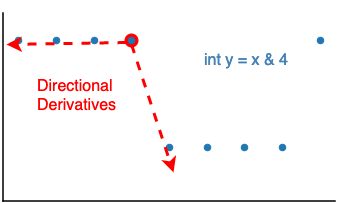
\includegraphics[width=0.7\columnwidth]{figs/directional_deriv_example}
  %\caption{\label{fig:dir_deriv} Directional derivative applied to a nonconvex function \tc{x \& 4}.}
%\end{figure}

We denote a generalized directional derivative in a directon $v$ as $f^\circ \left(x;v\right)$, which is formally defined as follows:

\vspace{-10pt}\begin{align}
  f^\circ \left(\bar{x}; v\right) = \lim \sup_{x \rightarrow \bar{x}, \lambda \downarrow 0} \frac{f\left(x + \lambda v\right) - f\left(x\right)}{\lambda}
\end{align}

\noindent Here $\bar{x}$ is the point at which the directional derivative is evaluated, $x$ can be any other point in the domain of $f$, and $\lambda$ is a distance along the vector $v$ that the derivative is taken in. The $\lim \sup_{x \rightarrow \bar{x}}$ notation indicates that the directional deriviative takes on the largest possible value for the two points $x$ and $x+\lambda v$ closest to $\bar{x}$ in the function's domain. The generalized gradient at a given point is then the set of all generalized directional derivatives for all possible directions from that point.

\begin{figure}
  \centering
  \begin{subfigure}[b]{0.45\columnwidth}
    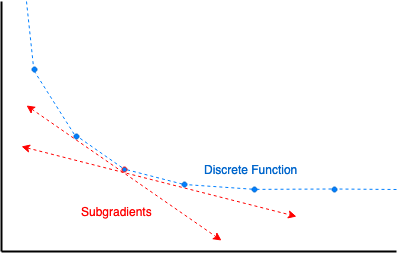
\includegraphics[width=\linewidth]{figs/subgradient_example}
    \caption{\label{fig:subgradient} Example of subgradient on discrete nonsmooth function.}
  \end{subfigure}
  \hspace{0.15cm}
  \begin{subfigure}[b]{0.5\columnwidth}
    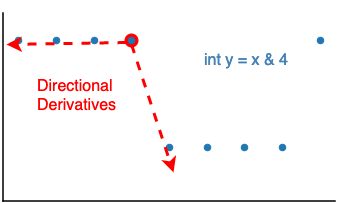
\includegraphics[width=\linewidth]{figs/directional_deriv_example}
  \caption{\label{fig:dir_deriv} Directional derivative applied to a nonconvex function \tc{x \& 4}.}
  \end{subfigure}
  \vspace{-10pt}
  \caption{\label{fig:grad_exs} Subgradient and Generalized Derivative examples.}
  \vspace{-15pt}
\end{figure}

\noindent \textbf{Lipschitz Continuity.} One important requirement of subgradients and generalized gradients is that the gradients of the functions they are computed over must be bounded. This property is called 'Lipschitz Continuity', and is defined as

\vspace{-10pt}\begin{align}
  |f\left(x_1\right) - f\left(x_0\right)| \leq K|x_1 - x_0|\\
  \textrm{ for all } x_1, x_0 \in x+\eta B \nonumber
\end{align}

\noindent where $K$, the Lipschitz Constant, is the bound on the gradient and $B$ denotes the size of the region in the domain of $f$ where the property is defined. Fortunately for the purpose of modeling programs, all operations ultimately occur on fixed width data types, limiting the range of values they can take on to the minimum and maximum of these data types and making them Lipschitz Continuous even in the worse case where a function jumps between extreme values.


\noindent \textbf{Proximal Gradients.} Subgradients and generalized gradients are useful guides analysis of discrete and nonconvex functions, but cannot be evaluated on general functions without sampling every possible value, which obviously isn't practical. To make evaluation tractable, we borrow another gradient approximation method from the discrete optimization literature called proximal gradients ~\cite{parikh2014proximal}. Instead of combining every possible surface or supporting vector under a function like subgradients and generalized gradients, proximal gradients use the minimum point within a soft bounded region. This region is defined by a cost function that increases quadratically with distance from the evaluation point. 

By representing the gradient with a single value and bounding the region in which it is evaluated, the proximal gradient makes the general problem of evaluating gradients tractable. The proximal operator is defined as follows when evaluated on a given point $\bar{x}$:

\vspace{-10pt}\begin{align}
  prox_f\left(\bar{x}\right) &= argmin_x \left(f\left(x\right) + \tfrac{1}{2}|| x-\bar{x}||_2^2\right)
\end{align}

The notation $argmin_x$ indicates that the operator selects the value of $x$ that minimizes both value of function $f\left(x\right)$ and the distance cost $\left(\tfrac{1}{2}\right)|| x-\bar{x}||_2^2$ that increases quadratically with the distance of $x$ from $\bar{x}$. Evaluating the proximal operator will give the minimum point near the point at which it is evaluated. This point can then be used to compute the largest directional derivative in the region near the point. 

% PROXIMAL GRADIENT
\vspace{-10pt}\begin{align}
  prox_{\nabla f}\left(\bar{x}\right) &= \frac{f\left(\bar{x}\right) - f\left(prox_f\left(\bar{x}\right)\right)}{\bar{x} - prox_f\left(\bar{x}\right)}
\end{align}

\noindent \textbf{Sampling Bounds.} On functions that are Lipschitz Continuous, the region that must be sampled to evaluate the proximal operator can be hard bounded as a factor of the Lipschitz Constant $K$. This bound is derived by observing that the cost function of the proximal operator is upper bounded by the initial function value and lower bounded by linear function decreasing at rate $K$ from the point $\bar{x}$ for $prox_f(\bar{x})$.

% BOUNDS DERIVATION 1
\vspace{-10pt}\begin{align*}
  \left(f\left(\bar{x}\right) - K*||prox_f\left(\bar{x}\right) - \bar{x}||_2  + \tfrac{1}{2}|| prox_f\left(\bar{x}\right)-\bar{x}||_2^2\right)\\
    \leq \left(f\left(prox_f\left(\bar{x}\right)\right) + \tfrac{1}{2}|| prox_f\left(\bar{x}\right)-\bar{x}||_2^2\right)\\
    \leq f\left(\bar{x}\right) + \tfrac{1}{2}||\bar{x} - \bar{x}||_2^2
\end{align*}

Here the term $f\left(\bar{x}\right) - K*||prox_f\left(\bar{x}\right)$ represents the minimum value $f$, can take as $prox_f\left(\bar{x}\right)$ moves farther from $\bar{x}$ due to its Lipschitz Constant $K$, while the value $f\left(\bar{x}\right) + \tfrac{1}{2}||\bar{x} - \bar{x}||_2^2$ represents the value being minimized at the initial point $\bar{x}$. This can be simplified by dropping the middle term: 

\vspace{-10pt}\begin{align*}
  \left(f(\bar{x}) - K*||prox_f\left(\bar{x}\right) - \bar{x}||_2  + \tfrac{1}{2}|| prox_f\left(\bar{x}\right)-\bar{x}||_2^2\right)\\
    \leq f\left(\bar{x}\right)
\end{align*}


as well as subtracting $f\left(\bar{x}\right)$ from both sides:

\vspace{-10pt}\begin{align*}
  \left( - K*||prox_f\left(\bar{x}\right) - \bar{x}||_2  + \tfrac{1}{2}|| prox_f\left(\bar{x}\right)-\bar{x}||_2^2\right) &\leq 0
\end{align*}

Adding $K*||\bar{x}-x||_2$ to both sides, dividing by $||\bar{x}-x||$, and multiplying by 2 gives a bound of $2K$ on the distance between the inital point $\bar{x}$ and the proximal operator result $prox_f\left(\bar{x}\right)$. 


\vspace{-10pt}\begin{align}
    || prox_f(\bar{x})-\bar{x}||_2 &\leq 2K
\end{align}

This means that the distance the result of the proximal operator from its initial $\bar{x}$ is bounded by at most twice the Lipschitz Constant for the function, $2K$. In practice a scaling factor $\lambda$ is often used with the proximal operator to adjust the relative weighting of distance from the evaluation point. When the scaling factor is added the bound becomes $2 \lambda K$. We then denote the Proximal Operator with a Lipschitz sampling bound $K$ and scaling factor $\lambda$ as

\vspace{-10pt}\begin{align}
  prox_f\left(\bar{x}, K, \lambda\right) &= argmin_x \left(f\left(x\right) + \tfrac{1}{2\lambda}|| x-\bar{x}||_2^2\right) \nonumber\\
  \textrm{s.t. } &|| x-\bar{x}||_2 \leq 2 \lambda K
\end{align}

\noindent and the associated bounded Proximal Gradient is:

\vspace{-10pt}\begin{align}
prox_{\nabla f}\left(\bar{x}, K, \lambda\right) &= \frac{f\left(\bar{x}\right) - f\left(prox_f\left(\bar{x}, K, \lambda\right)\right)}{\bar{x} - prox_f\left(\bar{x}, K, \lambda\right)}
\end{align}

This provides theoretically sound and adjustable method for bounding the sampling region on Lipschitz Continuous functions when the Lipschitz Constant $K$ is known.


\gabe{Probably should also explain smoothing here}

\subsection{Automatic Gradient Computation}

Automatically computing gradients over programs composed of analytically differentiable operations is a process called Automatic Differentiation, or 'AutoDiff', that has been a longstanding tool in computational modeling and is a core component of deep learning frameworks such as Tensorflow ~\cite{Wengert:1964:SAD:355586.364791, tensorflow2015-whitepaper}. Autodiff makes use of the chain rule in calculus to compute the gradient over a program as a series of gradients of individual operations multiplied together, each of which can be computed analytically. However, AutoDiff methods and frameworks have traditionally limited themselves to working with  functions that are at minimum piecewise differentiable, and do not support nonsmooth operations found in general programs such as bitwise operations or merge operations. By leveraging proximal gradients, the Autodiff approach can be extended to work with nonsmooth operations as well, thereby making it possible to compute gradients over general programs.



